\documentclass[border=10pt]{standalone}
\usepackage{tikz}\usepackage{amsmath}\usetikzlibrary{calc,arrows.meta}
\begin{document}
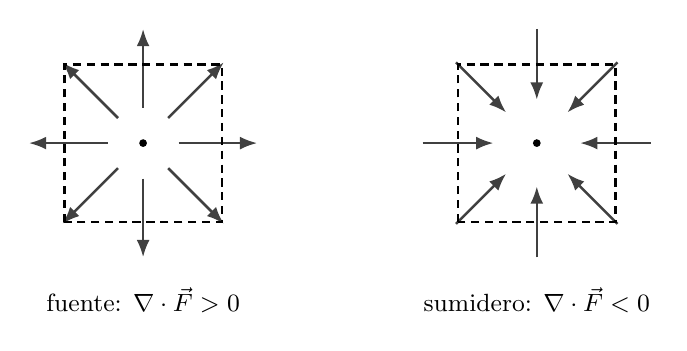
\begin{tikzpicture}[line width=0.9pt,>={Latex[length=2.2mm]}]
  % fuente
  \fill (0,0) circle(1.4pt);
  \foreach \a in {0,45,...,315} \draw[->,black!75] (\a:0.45)--(\a:1.45);
  \draw[densely dashed] (-1.0,-1.0) rectangle (1.0,1.0);
  \node at (0,-2.0){\small fuente: $\nabla\cdot\vec F>0$};
  % sumidero
  \begin{scope}[xshift=5cm]
    \fill (0,0) circle(1.4pt);
    \foreach \a in {0,45,...,315} \draw[->,black!75] (\a:1.45)--(\a:0.55);
    \draw[densely dashed] (-1.0,-1.0) rectangle (1.0,1.0);
    \node at (0,-2.0){\small sumidero: $\nabla\cdot\vec F<0$};
  \end{scope}
\end{tikzpicture}
\end{document}
